% !TeX program = lualatex

\documentclass[12pt]{report}
\usepackage[Glenn]{fncychap}
\usepackage[T1]{fontenc}
\usepackage[francais]{babel}
\usepackage{fontspec}
\usepackage{wrapfig}
\usepackage{graphicx}
\usepackage{soul}
\usepackage[colorlinks=true, linkcolor=black, urlcolor=black, citecolor=black]{hyperref}
% \usepackage[hyphens, spaces, obeyspaces]{url}
\usepackage[a4paper, width=175mm, top=25mm, bottom=25mm]{geometry}
\usepackage{parskip}
\usepackage{enumitem}
\usepackage{titlesec}
\usepackage{listings}
\usepackage{float}
\usepackage[final]{pdfpages}
\usepackage{xcolor}
\usepackage{tocbibind}
\usepackage{tocloft}
\usepackage{xpatch}
\usepackage{amsmath}
\usepackage{amsthm}
\usepackage{amsfonts}
\usepackage{graphics}
\usepackage{color}
% \usepackage[grey,utopia]{quotchap}
\usepackage{moreverb}
\usepackage{xcolor}
\usepackage{framed}
\usepackage{arabluatex}
%\usepackage[algo2e, french, onelanguage, ruled]{algorithm2e}
\setlist[itemize]{label=\textbullet}
\usepackage{fancyhdr}
\pagestyle{fancy}   
\fancyhead{}
\fancyhead[C]{\leftmark}
\renewcommand{\headrulewidth}{0.4pt}
\renewcommand{\footrulewidth}{0.4pt}
\usepackage{xcolor}
\definecolor{light-gray}{gray}{0.90}
\usepackage{multirow}
\usepackage{soul}
\usepackage{graphicx}
\usepackage[utf8x]{inputenc}
\setcounter{secnumdepth}{3} 
\usepackage{dirtytalk}
\usepackage{csquotes}
\usepackage{mathtools}
\usepackage{amsmath}
\begin{document}
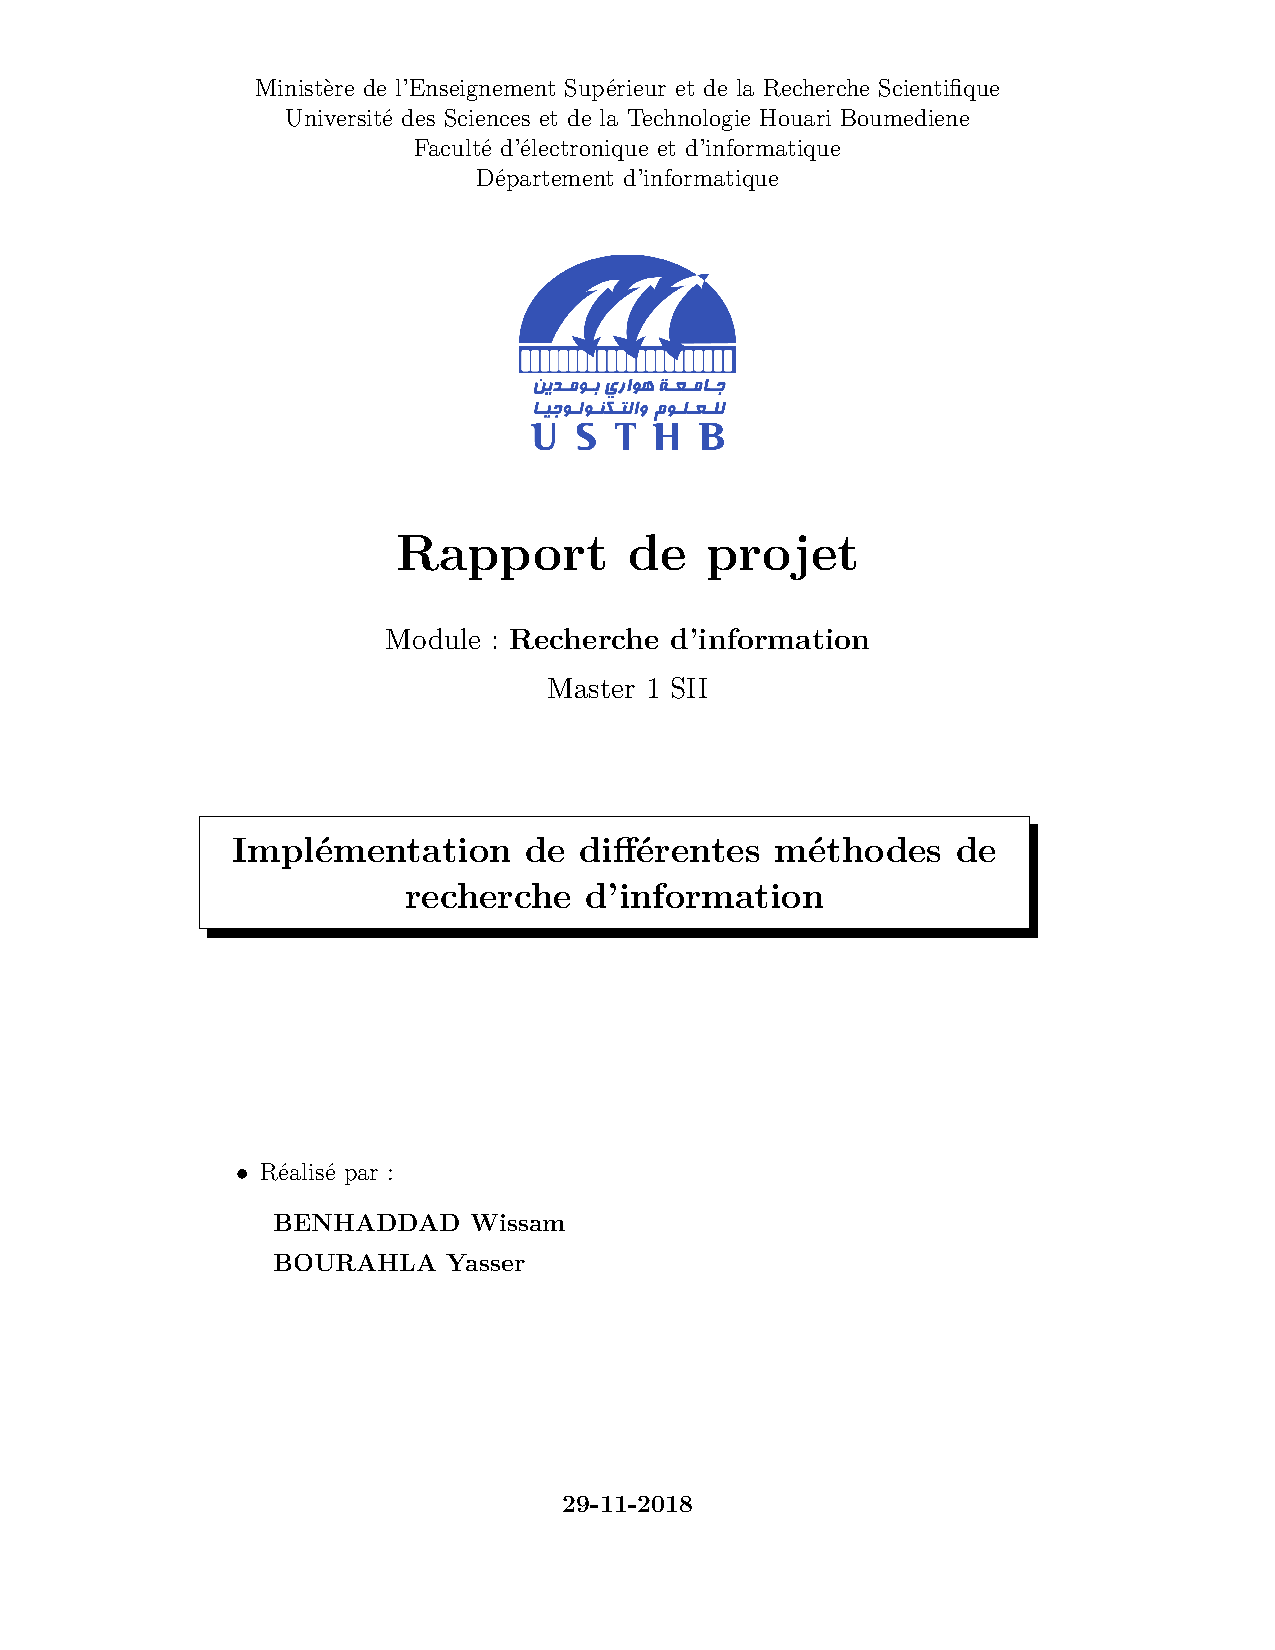
\includepdf[pages=1]{Page_garde.pdf} 
\tableofcontents
\listoffigures
\listoftables


\pagenumbering{arabic}
\newpage
%\title{Réalisation d'un assistant virtuel intelligent pour ordinateurs}
%\author{W.Benhaddad, Y.Bourahla}

\setlist[itemize]{label=\textbullet}



\chapter{Introduction}
	\section{Problématique et objectifs}
	\paragraph{}
	Talk about why we are gonna do this stuff.
	
	\section{Définitions}
	\paragraph{}
	Some definitions of the concepts,techniques and algorithms that we will use
		\subsection{La recherche d'information}
		\paragraph{}
		
		\subsection{L'indexation de documents}
		\paragraph{}
		
		\subsection{Méthodes de recherche}
			\subsubsection{Modèle booléen}
			\paragraph{}
			
			\subsubsection{Modèle Vectoriel}
			\paragraph{}
			
			\subsubsection{Modèle Probabiliste}
			\paragraph{}
		
	\section{Conclusion}
	
\chapter{Solution proposées et implémentation}
	\section{Outils utilisés}
		\subsection{Environnement de travail}
		\subsection{Langage}
		\subsection{Qt framework}
		
	\section{Schéma global du système}
	LET ME DO THE DIAGRAMS IF YOU DON'T WANNA
	
	\section{Implémentation et évaluation du modèle booléen}
	
	\section{Implémentation et évaluation du modèle vectoriel}
	
	\section{Implémentation et évaluation du modèle probabiliste}
	
	
	\section{Conclusion}
	Kheliahli rak ta3ref xD 
	
	
\chapter{Présentation de l'application}

	\section{Diagramme d'utilisation}
	\section{Exemples d'utilisation}
	
\chapter{Conclusion générale}
	\section{Comparaison des différentes méthodes}
	


\end{document}}

